% fig2-pipeline.tex — Figure 2: review pipeline overview (system overview)
\documentclass[tikz,border=10pt]{standalone}
\usetikzlibrary{arrows.meta,positioning,shapes.geometric,fit,backgrounds,calc}

\begin{document}
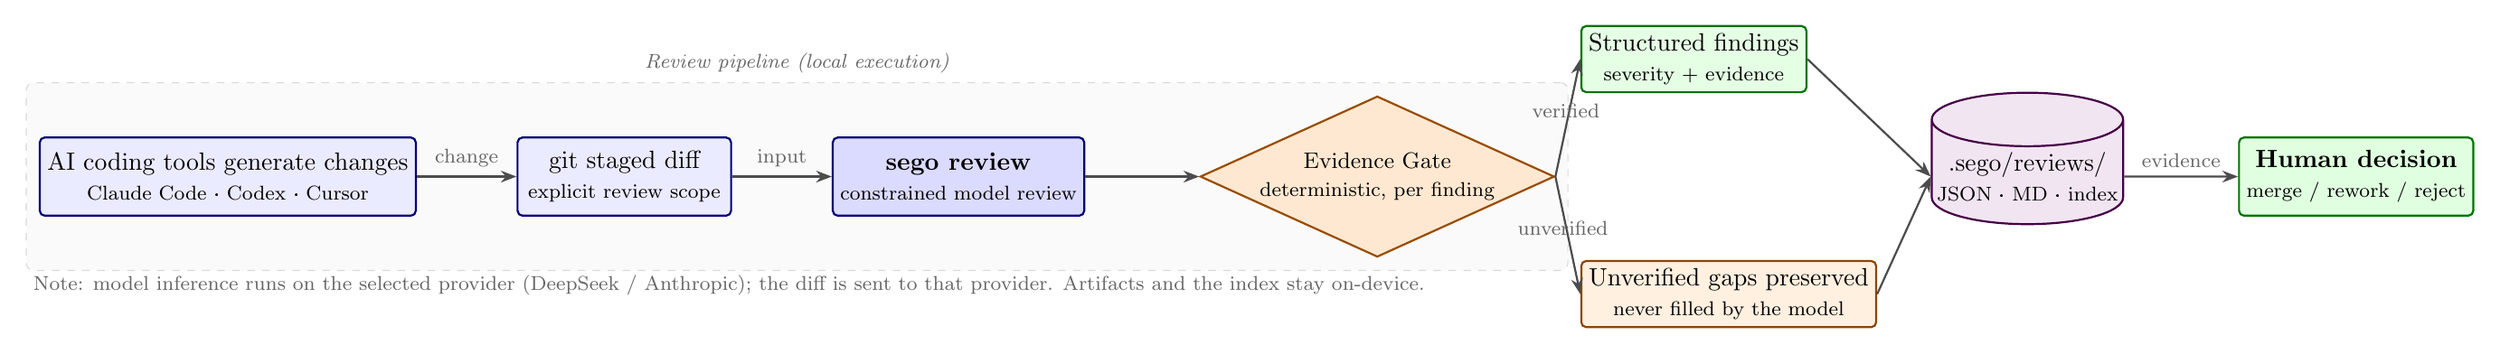
\begin{tikzpicture}[
  font=\normalsize,
  stage/.style={draw, rounded corners=2pt, thick, fill=blue!8, draw=blue!45!black,
                minimum width=30mm, minimum height=11mm, align=center, inner sep=3pt},
  gate/.style={draw, diamond, aspect=2.2, thick, fill=orange!18, draw=orange!60!black,
               align=center, inner sep=1pt, font=\small},
  outcome/.style={draw, rounded corners=2pt, thick, align=center, inner sep=3pt},
  store/.style={draw, cylinder, shape border rotate=90, aspect=0.28, thick,
                fill=violet!10, draw=violet!55!black, align=center, inner sep=2pt},
  human/.style={draw, rounded corners=2pt, thick, fill=green!12, draw=green!45!black,
                minimum height=11mm, align=center, inner sep=3pt},
  lab/.style={font=\footnotesize, text=black!60},
  arr/.style={-{Stealth[length=2.2mm]}, thick, draw=black!70}
]

\node[stage] (gen) {AI coding tools generate changes\\ \footnotesize Claude Code · Codex · Cursor};
\node[stage, right=14mm of gen] (diff) {git staged diff\\ \footnotesize explicit review scope};
\node[stage, right=14mm of diff, fill=blue!14] (review) {\textbf{sego review}\\ \footnotesize constrained model review};
\node[gate,  right=16mm of review] (gate) {Evidence Gate\\ \footnotesize deterministic, per finding};

\node[outcome, above right=6mm and 16mm of gate, fill=green!10, draw=green!45!black] (find)
  {Structured findings\\ \footnotesize severity + evidence};
\node[outcome, below right=6mm and 16mm of gate, fill=orange!12, draw=orange!55!black] (gap)
  {Unverified gaps preserved\\ \footnotesize never filled by the model};

\node[store] (art) at ($(find.east)!0.5!(gap.east) + (26mm, 0)$)
  {.sego/reviews/\\ \footnotesize JSON · MD · index};

\node[human, right=16mm of art] (human)
  {\textbf{Human decision}\\ \footnotesize merge / rework / reject};

\draw[arr] (gen)   -- node[lab, above] {change} (diff);
\draw[arr] (diff)  -- node[lab, above] {input} (review);
\draw[arr] (review)-- (gate);
\draw[arr] (gate.east) -- node[lab, above, pos=0.42] {verified} (find.west);
\draw[arr] (gate.east) -- node[lab, below, pos=0.30] {unverified} (gap.west);
\draw[arr] (find.east) -- (art.west);
\draw[arr] (gap.east) -- (art.west);
\draw[arr] (art) -- node[lab, above] {evidence} (human);

\begin{scope}[on background layer]
  \node[draw=black!15, dashed, rounded corners=3pt, fill=black!2,
        fit=(gen)(review)(gate), inner sep=5pt,
        label={[font=\footnotesize\itshape, text=black!60]above:Review pipeline (local execution)}] {};
\end{scope}

\node[lab, anchor=north west] at ($(gen.south west)+(-2mm,-7mm)$)
  {Note: model inference runs on the selected provider (DeepSeek / Anthropic); the diff is sent to that provider. Artifacts and the index stay on-device.};
\end{tikzpicture}
\end{document}
